\part*{Appendices}
%%CF.6.3: I don't think this is needed

\section{Pseudocode of CDS}
\label{app:alg}
We present the summary of the pseudocode of CDS in Algorithm~\ref{alg:cds}.
\vspace{-0.35cm}
\begin{algorithm}[H]
\begin{small}
  \caption{\methodname: Conservative Data Sharing}\label{alg:cds}
  \begin{algorithmic}[1]
    \REQUIRE Multi-task offline dataset $\cup_{i=1}^N \mathcal{D}_i$.
    \STATE Randomly initialize policy  $\pi_\theta(\ba|\bs, i)$.
    \FOR{$k=1, 2, 3, \cdots,$}
    \STATE Initialize $\mathcal{D}^\mathrm{eff} \leftarrow \{\}$
    \FOR{$i=1, \cdots, N$}
        \STATE $\mathcal{D}^\mathrm{eff}_i$ = $\mathcal{D}_i \cup \{(\bs_j, \ba_j, \bs'_j, r_i) \in \mathcal{D}_{j \rightarrow i}: \Delta^\pi(\bs, \ba) \geq 0\}$ using Eq.~\ref{eqn:method} (\methodname) or Eq.~\ref{eqn:p-cds} (\methodname (basic)).
    \ENDFOR
    \STATE Improve policy by solving eq.~\ref{eqn:generic_multitask_offline_rl} using samples from $\mathcal{D}^\mathrm{eff}$ to obtain $\policy_\theta^{k+1}$.
    \ENDFOR
  \end{algorithmic}
\end{small}
\end{algorithm}
\vspace{-0.5cm}

\section{Analysis of \methodname}
\label{app:proofs}

In this section, we will analyze the key idea behind our method \methodname\ (Section~\ref{sec:method}) and show that the abstract version of our method (Equation~\ref{eqn:optimize_behavior}) provides better policy improvement guarantees than na\"ive data sharing and that the practical version of our method (Equation~\ref{eqn:method}) approximates Equation~\ref{eqn:optimize_behavior} resulting in an effective practical algorithm.

\subsection{Analysis of the Algorithm in Equation~\ref{eqn:optimize_behavior}}
We begin with analyzing Equation~\ref{eqn:optimize_behavior},
which is used to derive the practical variant of our method, \methodname. We build on the analysis of safe-policy improvement guarantees of conventional offline RL algorithms~\citep{laroche2019safe,kumar2020conservative} and show that data sharing using \methodname\ attains better guarantees in the worst case. To begin the analysis, we introduce some notation and prior results that we will directly compare to.

\textbf{Notation and prior results.}
%%CF.6.3: you have a paragraph header here, but then don't have a paragraph header when you start talking about things that aren't notation and prior results?
Let $\pi_\beta(\ba|\bs)$ denote the behavior policy for task $i$ (note that index $i$ was dropped from $\pi_\beta(\ba|\bs; i)$ for brevity). The dataset, $\mathcal{D}_i$ 
is generated from the marginal state-action distribution of $\pi_\beta$, i.e., $\mathcal{D} \sim d^{\pi_\beta}(\bs) \pi_\beta(\ba|\bs)$. We define $d^{\pi}_{\mathcal{D}}$ as the state marginal distribution introduced by the dataset $\mathcal{D}$ under $\pi$. Let $D_\text{CQL}(p, q)$ denote the following distance between two distributions $p(\bx)$ and $q(\bx)$ with equal support $\mathcal{X}$:
\begin{equation*}
    D_\text{CQL}(p, q) := \sum_{\bx \in \mathcal{X}} p(\bx) \left(\frac{p(\bx)}{q(\bx)} - 1 \right).
\end{equation*}
Unless otherwise mentioned, we will drop the subscript ``CQL'' from $D_\text{CQL}$ and use $D$ and $D_\text{CQL}$ interchangeably. Prior works~\citep{kumar2020conservative} have shown that the optimal policy $\pi^*_{i}$ that optimizes Equation~\ref{eqn:generic_offline_rl} attains a high probability safe-policy improvement guarantee, i.e., $J(\pi^*_i) \geq J(\pi_\beta) - \zeta_i$, where $\zeta_i$ is:
\begin{equation}
    \label{eqn:single_task_guarantee}
    \zeta_i =  \mathcal{O}\left(\frac{1}{(1 - \gamma)^2}\right) \mathbb{E}_{\bs \sim d^{\pi^*_i}_{\mathcal{D}_i}}\left[\sqrt{\frac{D_{\text{CQL}}(\pi^*_i, \pi_\beta)(\bs) + 1}{|\mathcal{D}_i(\bs)|}} \right] + \alpha D(\pi^*_i, \pi_\beta).
\end{equation}
The first term in Equation~\ref{eqn:single_task_guarantee} corresponds to the decrease in performance due to sampling error and this term is high when the single-task optimal policy $\pi^*_i$ visits rarely observed states in the dataset $\mathcal{D}_i$ and/or when the divergence from the behavior policy $\pi_\beta$ is higher under the states visited by the single-task policy $\bs \sim d^{\pi^*_i}_{\mathcal{D}_i}$. 

Let $J_\mathcal{D}(\pi)$ denote the return of a policy $\pi$ in the empirical MDP induced by the transitions in the dataset $\mathcal{D}$. Further, let us assume that optimizing Equation~\ref{eqn:optimize_behavior} gives us the following policies:
\begin{equation}
    \label{eqn:eqn4_detailed}
    \pi^*(\ba|\bs), \pi^*_\beta(\ba|\bs) := \arg \max_{\pi, \pi_\beta \in \Pi_{\text{relabel}}}~~ \underbrace{J_{\mathcal{D}^\mathrm{eff}_i}(\pi) - \alpha D(\pi, \pi_\beta)}_{:= f(\pi, \pi_\beta; \mathcal{D}^\mathrm{eff}_i)},
\end{equation}
where the optimized behavior policy $\pi^*_\beta$ is constrained to lie in a set of all policies that can be obtained via relabeling, $\Pi_\text{relabel}$, and the dataset, $\mathcal{D}^\mathrm{eff}_i$ is sampled according to the state-action marginal distribution of $\pi^*_\beta$, i.e., $\mathcal{D}^\mathrm{eff}_i \sim d^{\pi^*_\beta}(\bs, \ba)$. Additionally, for convenience, define, $f(\pi_1, \pi_2; \mathcal{D}) := J_\mathcal{D}(\pi_1) - \alpha D(\pi_1, \pi_2)$ for any two policies $\pi_1$ and $\pi_2$, and a given dataset $\mathcal{D}$. 

We now show the following result for \methodname:

\begin{proposition}[Proposition~\ref{prop:spi_thm} restated] 
\label{prop:spi}
Let $\pi^*(\ba|\bs)$ be the policy obtained by optimizing Equation~\ref{eqn:optimize_behavior}, and let $\pi_\beta(\ba|\bs)$ be the behavior policy for $\mathcal{D}_i$. Then, w.h.p. $\geq 1 - \delta$, $\pi^*$ is a $\zeta$-safe policy improvement over $\pi_\beta$, i.e., $J(\pi^*) \geq J(\pi_\beta) - \zeta$, where $\zeta$ is given by:
\begin{equation*}
    \zeta = \mathcal{O}\left(\frac{1}{(1 - \gamma)^2}\right) \mathbb{E}_{\bs \sim d^{\pi^*}_{\mathcal{D}^\mathrm{eff}_i}}\left[\sqrt{\frac{D_{\text{CQL}}(\pi^*, \pi_\beta^*)(\bs) + 1}{|\mathcal{D}^\mathrm{eff}_i(\bs)|}} \right] -  \left[\alpha D(\pi^*, \pi_\beta^*) + \underbrace{J(\pi^*_\beta) - J(\pi_\beta)}_{\text{(a)}} \right],
\end{equation*}
where $\mathcal{D}^\mathrm{eff}_i \sim d^{\pi_\beta^*}(\bs)$ and $\pi^*_\beta(\ba|\bs)$ denotes the policy $\pi \in \Pi_{\text{relabel}}$ that maximizes Equation~\ref{eqn:optimize_behavior}. 
\end{proposition}
\begin{proof}
To prove this proposition, we shall quantify the lower-bound on the improvement in the policy performance due to Equation~\ref{eqn:eqn4_detailed} in the empirical MDP, and the potential drop in policy performance in the original MDP due to sampling error, and combine the terms to obtain our bound. First note that for any given policy $\pi$, and a dataset $\mathcal{D}^\mathrm{eff}_i$ with effective behavior policy $\pi_\beta(\ba|\bs)$, the following bound holds~\citep{kumar2020conservative}:
\begin{equation}
\label{eqn:sampling_error}
    J(\pi) \geq J_{\mathcal{D}^\mathrm{eff}_i} (\pi) - \mathcal{O}\left(\frac{1}{(1 - \gamma)^2}\right) \mathbb{E}_{\bs \sim d^{\pi}_{\mathcal{D}^\mathrm{eff}_i}}\left[\sqrt{\frac{D_{\text{CQL}}(\pi, \pi^*_\beta)(\bs) + 1}{|\mathcal{D}^\mathrm{eff}_i(\bs)|}} \right],
\end{equation}
where the $\mathcal{O}(\cdot)$ notation hides constants depending upon the concentration properties of the MDP~\citep{laroche2019safe} and $1 - \delta$, the probability with which the statement holds. Next, we provide guarantees on policy improvement in the empirical MDP. To see this, note that the following statements on $f(\pi_1, \pi_2; \mathcal{D})$ are true:
\begin{align}
    &\forall \pi' \in \Pi_{\text{relabel}}, ~~f(\pi^*, \pi^*_\beta; \mathcal{D}^\mathrm{eff}_i) \geq f(\pi', \pi', \mathcal{D}^\mathrm{eff}_i)\\
    \implies & \forall \pi' \in \Pi_{\text{relabel}},~~ J_{\mathcal{D}^\mathrm{eff}_i}(\pi^*) - \alpha D(\pi^*, \pi^*_\beta) \geq J_{\mathcal{D}^\mathrm{eff}_i}(\pi').
    \label{eqn:inequality_policy}
\end{align}
And additionally, we obtain:
\begin{align}
    &\forall \pi' \in \Pi_\text{relabel}, ~~f(\pi^*, \pi^*_\beta; \mathcal{D}^\mathrm{eff}_i) \geq f(\pi^*, \pi'; \mathcal{D}^\mathrm{eff}_i),\\
    \implies &\forall \pi' \in \Pi_\text{relabel},~~ D(\pi^*, \pi^*_\beta) \leq D(\pi^*, \pi').
\end{align}
Utilizing \ref{eqn:inequality_policy}, we obtain that:
\begin{equation}
\label{eqn:perf_increase}
   J_{\mathcal{D}^\mathrm{eff}_i}(\pi^*) - J_{\mathcal{D}^\mathrm{eff}_i}(\pi_\beta) \geq \alpha D(\pi^*, \pi^*_\beta) + \left( J_{\mathcal{D}^\mathrm{eff}_i}(\pi_\beta^*) - J_{\mathcal{D}^\mathrm{eff}_i}(\pi_\beta) \right) \approx \alpha D(\pi^*, \pi^*_\beta) + \left(J(\pi^*_\beta) - J(\pi_\beta) \right),
\end{equation}
where $\approx$ ignores sampling error terms that do not depend on distributional shift measures like $D_\text{CQL}$ because $\pi^*_\beta$ and $\pi_\beta$ are behavior policies which generated the complete and part of the dataset, and hence these terms are dominated by and subsumed into the sampling error for $\pi^*$. Combining Equations~\ref{eqn:sampling_error} (by setting $\pi = \pi^*$) and \ref{eqn:perf_increase}, we obtain the following safe-policy improvement guarantee for $\pi^*$: $J(\pi^*) - J(\pi_\beta) \geq \zeta$, where $\zeta$ is given by:
\begin{equation*}
    \zeta = \mathcal{O}\left(\frac{1}{(1 - \gamma)^2}\right) \mathbb{E}_{\bs \sim d^{\pi^*}_{\mathcal{D}^\mathrm{eff}_i}}\left[\sqrt{\frac{D_{\text{CQL}}(\pi^*, \pi_\beta^*)(\bs) + 1}{|\mathcal{D}^\mathrm{eff}_i(\bs)|}} \right] -  \left[\alpha D(\pi^*, \pi_\beta^*) + \underbrace{J(\pi^*_\beta) - J(\pi_\beta)}_{\text{(a)}} \right],
\end{equation*}
which proves the desired result.
\end{proof}
Proposition~\ref{prop:spi} indicates that when optimizing the behavior policy with Equation~\ref{eqn:optimize_behavior}, we can improve upon the conventional safe-policy improvement guarantee (Equation~\ref{eqn:single_task_guarantee}) with standard single-task offline RL: not only do we improve via $D_\text{CQL}(\pi^*, \pi_\beta^*)$, since, $D_\text{CQL}(\pi^*, \pi_\beta^*) \leq D_\text{CQL}(\pi^*, \pi_\beta)$, which reduces sampling error, but utilizing this policy $\pi^*_\beta$ also allows us to improve on term $(a)$, since Equation~\ref{eqn:eqn4_detailed} optimizes the behavior policy to be close to the learned policy $\pi^*$ and maximizes the learned policy return $J_{\mathcal{D}^\mathrm{eff}_i}(\pi^*)$ on the effective dataset, thus providing us with a high lower bound on $J(\pi^*_\beta)$. We formalize this insight as Lemma~\ref{lemma:a_gt_0} below:

\begin{lemma}
\label{lemma:a_gt_0}
For sufficiently large $\alpha$, $J_{\mathcal{D}^\mathrm{eff}_i}(\pi^*_\beta) \geq J_{\mathcal{D}^\mathrm{eff}_i}(\pi_\beta)$ and thus $(a) \geq 0$.
\end{lemma}
\begin{proof}
To prove this, we note that using standard difference of returns of two policies, we get the following inequality: $J_{\mathcal{D}^\mathrm{eff}_i}(\pi^*_\beta) \geq J_{\mathcal{D}^\mathrm{eff}_i}(\pi^*) - C \frac{R_{\max}}{1 - \gamma} D_{\mathrm{TV}}(\pi^*, \pi^*_\beta)$. Moreover, from Equation~\ref{eqn:inequality_policy}, we obtain that: $J_{\mathcal{D}^\mathrm{eff}_i}(\pi^*) - \alpha D(\pi^*, \pi^*_\beta) \geq J_{\mathcal{D}^\mathrm{eff}_i}(\pi_\beta)$. So, if $\alpha$ is chosen such that:
\begin{equation}
    \frac{C R_{\max}}{1 - \gamma } D_\mathrm{TV}(\pi^*, \pi_\beta^*) \leq \alpha D(\pi^*, \pi^*_\beta),
\end{equation}
we find that:
\begin{equation*}
    J_{\mathcal{D}^\mathrm{eff}_i}(\pi^*_\beta) \geq J_{\mathcal{D}^\mathrm{eff}_i}(\pi^*) - C \frac{R_{\max}}{1 - \gamma} D_{\mathrm{TV}}(\pi^*, \pi^*_\beta) \geq J_{\mathcal{D}^\mathrm{eff}_i}(\pi^*) - \alpha D(\pi^*, \pi^*_\beta) \geq J_{\mathcal{D}^\mathrm{eff}_i}(\pi_\beta),
\end{equation*}
implying that $(a) \geq 0$. For the edge cases when either $D_\mathrm{TV}(\pi^*, \pi^*_\beta) = 0$ or $D_{\text{CQL}}(\pi^*, \pi^*_\beta) = 0$, we note that $\pi^*(\ba|\bs) = \pi^*_\beta(\ba|\bs)$, which trivially implies that $J_{\mathcal{D}^\mathrm{eff}_i}(\pi^*_\beta) = J_{\mathcal{D}^\mathrm{eff}_i}(\pi^*) \geq J_{\mathcal{D}^\mathrm{eff}_i}(\pi_\beta)$, because $\pi^*$ improves over $\pi_\beta$ on the dataset. Thus, term $(a)$ is positive for large-enough $\alpha$ and the bound in Proposition~\ref{prop:spi} gains from this term additionally.
\end{proof}

Finally, we show that the sampling error term is controlled when utilizing Equation~\ref{eqn:optimize_behavior}. We will show in Lemma~\ref{lemma:sampling_error} that the sampling error in Proposition~\ref{prop:spi} is controlled to be not much bigger than the error just due to variance, since distributional shift is bounded with Equation~\ref{eqn:optimize_behavior}.
\begin{lemma}
\label{lemma:sampling_error}
If $\pi^*$ and $\pi^*_\beta$ obtained from Equation~\ref{eqn:optimize_behavior} satisfy, $D_\text{CQL}(\pi^*, \pi^*_\beta) \leq \varepsilon \ll 1$, then:
\begin{equation}
    (\$) := \mathbb{E}_{\bs \sim d^{\pi^*}_{\mathcal{D}^\mathrm{eff}_i}}\left[\sqrt{\frac{D_{\text{CQL}}(\pi^*, \pi_\beta^*)(\bs) + 1}{|\mathcal{D}^\mathrm{eff}_i(\bs)|}} \right] \leq (1 + \varepsilon)^{\frac{1}{2}} \underbrace{\mathbb{E}_{\bs \sim d^{\pi^*}_{\mathcal{D}^\mathrm{eff}_i}}\left[\sqrt{\frac{1}{|\mathcal{D}^\mathrm{eff}_i(\bs)|}}~ \right]}_{:= \text{sampling error w/o distribution shift}}.
\end{equation}
\end{lemma}
\begin{proof}
This lemma can be proved via a simple application of the Cauchy-Schwarz inequality. We can partition the first term as a sum over dot products of two vectors such that:
\begin{align*}
    (\$) &= \sum_{\bs} \sqrt{d^{\pi^*}_{\mathcal{D}^\mathrm{eff}_i}(\bs) (D_{\text{CQL}}(\pi^*, \pi_\beta^*)(\bs) + 1)} \sqrt{\frac{d^{\pi^*}_{\mathcal{D}^\mathrm{eff}_i}(\bs)}{|\mathcal{D}^\mathrm{eff}_i(\bs)|}}\\
    &\leq \sqrt{\left( \sum_{\bs} d^{\pi^*}_{\mathcal{D}^\mathrm{eff}_i}(\bs) (D_{\text{CQL}}(\pi^*, \pi_\beta^*)(\bs) + 1) \right) \cdot \left( \sum_{\bs} \frac{d^{\pi^*}_{\mathcal{D}^\mathrm{eff}_i}(\bs)}{|\mathcal{D}^\mathrm{eff}_i(\bs)|} \right)}\\
    &= \sqrt{\mathbb{E}_{\bs \sim d^{\pi^*}_{\mathcal{D}^\mathrm{eff}_i}}\left[D_{\text{CQL}}(\pi^*, \pi_\beta^*)(\bs) + 1\right] \mathbb{E}_{\bs \sim d^{\pi^*}_{\mathcal{D}^\mathrm{eff}_i}}\left[ \frac{1}{|\mathcal{D}^\mathrm{eff}_i(\bs)|} \right]} \leq (1 + \varepsilon)^{0.5} \mathbb{E}_{\bs \sim d^{\pi^*}_{\mathcal{D}^\mathrm{eff}_i}}\left[\sqrt{\frac{1}{|\mathcal{D}^\mathrm{eff}_i(\bs)|}}~ \right],
\end{align*}
where we note that $\mathbb{E}_{\bs \sim d^{\pi^*}_{\mathcal{D}^\mathrm{eff}_i}}\left[D_{\text{CQL}}(\pi^*, \pi_\beta^*)(\bs)\right] = D_\text{CQL}(\pi^*, \pi^*_\beta) \leq \varepsilon$ (based on the given information in the Lemma) and that $\sqrt{\sum_i w_i \frac{1}{x_i}} \leq \sum_i w_i \frac{1}{\sqrt{x_i}}$ for $x_i, w_i > 0$ and $\sum_i w_i = 1$, via Jensen's inequality for concave functions.
\end{proof}

\textbf{To summarize,} combining Lemmas~\ref{lemma:a_gt_0} and \ref{lemma:sampling_error} with Proposition~\ref{prop:spi}, we conclude that utilizing Equation~\ref{eqn:optimize_behavior} controls the increase in sampling error due to distributional shift, and provides improvement guarantees on the learned policy beyond the behavior policy of the original dataset. We also briefly now discuss the comparison between \methodname\ and complete data sharing. Complete data sharing would try to reduce sampling error by increasing $|\mathcal{D}^\mathrm{eff}_i(\bs)|$, but then it can also increase distributional shift, $D_\text{CQL}(\pi^*, \pi^*_\beta)$ as discussed in Section~\ref{sec:analysis}. On the other hand, CDS increases the dataset size while also controlling for distributional shift (as we discussed in the analysis above), making it enjoy the benefits of complete data sharing and avoiding its pitfalls, intuitively. On the other hand, no data sharing will just incur high sampling error due to limited dataset size. 

\subsection{From Equation~\ref{eqn:optimize_behavior} to Practical \methodname\ (Equation~\ref{eqn:method})}
\label{sec:practical_cds}
The goal of our practical algorithm is to convert Equation~\ref{eqn:optimize_behavior} to a practical algorithm while retaining the policy improvement guarantees derived in Proposition~\ref{prop:spi}. Since our algorithm does not utilize any estimator for dataset counts $|\mathcal{D}^\mathrm{eff}_i(\bs)|$, and since we operate in a continuous state-action space, our goal is to retain the guarantees of increased return of $\pi^*_\beta$, while also avoiding sampling error. 

With this goal, we first need to relax the state-distribution in Equation~\ref{eqn:optimize_behavior}: while both $J_{\mathcal{D}^\mathrm{eff}_i}(\pi)$ and $D_\text{CQL}(\pi, \pi_\beta)$ are computed as expectations under the marginal state-distribution of policy $\pi(\ba|\bs)$ on the MDP defined by the dataset $\mathcal{D}^\mathrm{eff}_i$, for deriving a practical method we relax the state distribution to use the dataset state-distribution $d^{\pi^*_\beta}$ and rewrite the objective in accordance with most practical implementations of actor-critic algorithms~\citep{degris2012off,Abdolmaleki2018MaximumAP,haarnoja2018soft,fujimoto2018addressing,lillicrap2015continuous} below:
\begin{equation}
\label{eqn:practical_eqn4}
    \text{(Practical Equation~\ref{eqn:optimize_behavior})}~~~~ \max_{\pi} \max_{\pi_\beta \in \Pi_\text{relabel}}~~ \mathbb{E}_{\bs \sim \mathcal{D}^{\mathrm{eff}}_i}[\mathbb{E}_{\ba \sim \pi(\ba|\bs)}[Q(\bs, \ba)] - \alpha D(\pi(\cdot|\bs), \pi_\beta(\cdot|\bs))]
\end{equation}
This practical approximation in Equation~\ref{eqn:practical_eqn4} is even more justified with conservative RL algorithms when a large $\alpha$ is used, since a larger $\alpha$ implies a smaller value for $D(\pi^*, \pi_\beta^*)$ found by Equation~\ref{eqn:optimize_behavior}, which in turn means that state-distributions $d^{\pi_\beta^*}$ and $d^{\pi^*}$ are close to each other~\citep{schulman2015trust}. Thus, our policy improvement objective optimizes the policies $\pi$ and $\pi_\beta$ by maximizing the conservative Q-function: $\hat{Q}^\pi(\bs, \ba) = Q(\bs, \ba) - \alpha \left(\frac{\pi(\ba|\bs)}{\pi_\beta(\ba|\bs)} - 1 \right)$, that appears inside the expectation in Equation~\ref{eqn:practical_eqn4}. While optimizing the policy $\pi$ with respect to this conservative Q-function $\hat{Q}^\pi(\bs, \ba)$ is equivalent to a standard policy improvement update utilized by most actor-critic methods~\citep{fujimoto2018addressing,haarnoja2018soft,kumar2020conservative}, we can optimize $\hat{Q}^\pi(\bs, \ba)$ with respect to $\pi_\beta \in \Pi_{\text{relabel}}$ by relabeling only those transitions $(\bs, \ba, r'_i, \bs') \in \mathcal{D}_{j \rightarrow i}$ that increase the expected conservative Q-value $\mathbb{E}_{\bs \sim \mathcal{D}^\mathrm{eff}_i}\left[\mathbb{E}_{\ba \sim \pi_\beta(\cdot|\bs)}\left[\hat{Q}^\pi(\bs, \ba)\right] \right]$. Note that we relaxed the expectation $\ba \sim \pi(\ba|\bs)$ to $\ba \sim \pi_\beta(\ba|\bs)$ in this expectation, which can be done upto a lower-bound of the objective in Equation~\ref{eqn:practical_eqn4} for a large $\alpha$, since the resulting policies $\pi$ and $\pi_\beta$ are close to each other.  

The last step in our practical algorithm is to modify the solution of Equation~\ref{eqn:practical_eqn4} to still retain the benefits of reduced sampling error as discussed in Proposition~\ref{prop:spi}. To do so, we want to relabel as many points as possible, thus increasing $|\mathcal{D}^\mathrm{eff}_i(\bs)|$, which leads to reduced sampling error. Since quantifying $|\mathcal{D}^\mathrm{eff}_i(\bs)|$ in continuous state-action spaces will require additional machinery such as density-models, we avoid these for the sake of simplicity, and instead choose to relabel every datapoint $(\bs, \ba) \in \mathcal{D}_{j \rightarrow i}$ that satisfies $Q^\pi(\bs, \ba; i) \geq \mathbb{E}_{\bs, \ba \sim \mathcal{D}_i}[\hat{Q}^\pi(\bs, \ba; i)] \geq 0$ to task $i$. These datapoints definitely increase the conservative Q-value and hence increase the objective in Equation~\ref{eqn:practical_eqn4} (though do not globally maximize it), while also enjoying properties of reduced sampling error (Proposition~\ref{prop:spi}). This discussion motivates our practical algorithm in Equation~\ref{eqn:method}.  

\section{Experimental details}
\label{app:details}

In this section, we provide the training details of CDS in Appendix~\ref{app:training_details} and also include the details on the environment and datasets that we use for the evaluation in Appendix~\ref{app:env_data_details}. Finally, we include the discussion on the compute information in Appendix~\ref{app:compute_details}. \arxiv{We also compare CDS to an offline RL with pretrained representations from multi-task datasets method~\citep{yang2021representation}.}

\subsection{Training details}
\label{app:training_details}

The pseudocode of CDS is summarized in Algorithm~\ref{alg:cds} in Appendix~\ref{app:alg}. The complete variant of CDS can be directly implemented using the rule in Equation~\ref{eqn:method} with conservative Q-value estimates obtained via any offline RL method that constrains the learned policy to the behavior policy. For implementing \methodname\ (basic), we reparameterize the divergence $D$ in Equation~\ref{eqn:pessimistically_conservative} to use the learned conservative Q-values. This is especially useful for our implementation since we utilize CQL as the base offline RL method, and hence we do not have access to an explicit divergence. In this case, $\Delta^\pi(\bs, \ba)$ can be redefined as, $\Delta^\pi(\bs, \ba) :=$
\begin{align}
    \mathbb{E}_{\bs' \sim \mathcal{D}^i}\left[\mathbb{E}_{\ba' \sim \pi}[\hat{Q}(\bs', \ba', i)] - \mathbb{E}_{\ba'' \sim \mathcal{D}_i}[\hat{Q}(\bs', \ba'', i)]\right] - \left(\mathbb{E}_{\ba' \sim \pi}[\hat{Q}(\bs, \ba', i)] - Q(\bs, \ba, i)\right),
\label{eqn:p-cds}
\end{align}
% \begin{align}
%     \Delta^\pi(\bs, \ba)  := 
%     -\left(\mathbb{E}_{\ba \sim \mu(\cdot|\bs)}\!\left[Q(\bs,\ba, i)\right]\!-\!\mathbb{E}_{\bs', \ba' \sim \mathcal{D}_i}\!\left[Q(\bs',\ba', i)\right]\right) +
%     \left(\mathbb{E}_{\bs\sim \mathcal{D}_i, \ba \sim \mu(\cdot|\bs)}\!\left[Q(\bs,\ba, i)\right]\!-\!\mathbb{E}_{\bs', \ba' \sim \mathcal{D}_i}\!\left[Q(\bs',\ba', i)\right]\right)
% \label{eqn:p-cds}
% \end{align}
% where $\mu(\cdot|s)$ is a wide sampling distribution such as the uniform distribution over the range of actions.
Equation~\ref{eqn:p-cds} can be viewed as the difference between the CQL~\citep{kumar2020conservative} regularization term on a given $(\bs, \ba)$ and the original dataset for task $i$, $\mathcal{D}_i$. This CQL regularization term is equal to the divergence between the learned policy $\pi(\cdot|\bs)$ and the behavior policy $\pi_\beta(\cdot|\bs)$, therefore Equation~\ref{eqn:p-cds} practically computes Equation~\ref{eqn:pessimistically_conservative}. 
% Intuitively, if the condition in Equation~\ref{eqn:p-cds} is true for certain $(\bs, \ba)$, adding it to $\mathcal{D}^\mathrm{eff}_i$ would decrease the expected CQL regularization term, which estimates the distributional shift $D_\text{CQL}(\pi(\cdot|\cdot, i), \pi_\beta^{\text{eff}}(\cdot|\cdot, i))$.

Note that both variants of \methodname\ train a policy, 
$\pi(\ba|\bs; i)$, either conditioned on the task $i$ (i.e., with weight sharing) or a separate $\pi(\ba|\bs)$ policy for each task with no weight sharing, using the resulting relabeled dataset, $\mathcal{D}^\mathrm{eff}_i$. Next, we discuss the training details of the complete version of \methodname.

Our practical implementation of \methodname\ optimizes the following objectives for training the critic and the policy:
\vspace*{-5pt}
\begin{small}
\begin{align*}
    \hat{Q}^{k+1} \leftarrow& \arg\min_{\hat{Q}} \mathbb{E}_{i\sim[N]}\left[\beta\left(\mathbb{E}_{j \sim[N]}\left[\mathbb{E}_{\bs \sim \mathcal{D}_j, \ba \sim \mu(\cdot|\bs,i)}\left[w_{\mathrm{\methodname}}(\bs, \ba; j \rightarrow i)\hat{Q}(\bs,\ba,i)\right]\right.\right.\right.\\
    &\left.\left.\left.- \mathbb{E}_{\bs, \ba \sim \mathcal{D}_j}\left[w_{\mathrm{\methodname}}(\bs, \ba; j \rightarrow i)\hat{Q}(\bs,\ba, i)\right]\right]\right)\right.\\
    &\left. + \frac{1}{2}\mathbb{E}_{j\sim[N],(\bs, \ba, \bs') \sim \mathcal{D}_j}\left[w_{\mathrm{\methodname}}(\bs, \ba; j \rightarrow i) \left(\hat{Q}(\bs, \ba, i) - \widehat{\bellman}^\policy \hat{Q}^k(\bs, \ba, i)\right)^2 \right]\right],
\end{align*}
\end{small}
\vspace*{-19pt}
and
\[
\policy \leftarrow \arg \max_{\policy'} \ \mathbb{E}_{i \sim [N]}\left[\mathbb{E}_{j\sim[N],\bs \sim \mathcal{D}_j, \ba \sim \policy'(\cdot | \bs, i)} \left[ w_{\mathrm{\methodname}}(\bs, \ba; j \rightarrow i)\hat{Q}^\policy (\bs, \ba, i) \right]\right],
\]
where $\beta$ is the coefficient of the CQL penalty on distribution shift, $\mu$ is a wide sampling distribution as in CQL and $\widehat{\bellman}$ is the sample-based Bellman operator.

To compute the relabeling weight $w_{\mathrm{\methodname}}(\bs, \ba; j \rightarrow i) := \sigma \left(\frac{\Delta(\bs, \ba; j \rightarrow i)}{\tau} \right)$, we need to pick the value of the temperature term $\tau$. Instead of tuning $\tau$ manually, we follow the the adaptive temperature scaling scheme from \citep{kumar2020discor}. Specifically, we compute an exponential running average of $\Delta(\bs, \ba; j \rightarrow i)$ with decay $0.995$ for each task and use it as $\tau$. We additionally clip the adaptive temperature term with a minimum and maximum threshold, which we tune manually. For multi-task halfcheetah, walker2d and ant, we clip the adaptive temperature such that it lies within $[10,\infty]$, $[5,\infty]$ and $[10,25]$ respectively. For the multi-task Meta-Wold experiment, we use $[1, 50]$ for the clipping. For multi-task Antmaze, we used a range of $[10, \infty]$ for all the domains. We do not clip the temperature term on vision-based domains.

For state-based experiments, we use a stratified batch with $128$ transitions for each task for the critic and policy learning. For each task $i$, we sample $64$ transitions from $\mathcal{D}_i$ and another $64$ transitions from $\cup_{j \neq i} \mathcal{D}_{j \rightarrow i}$, i.e. the relabeled datasets of all the other tasks. When computing $\Delta(\bs, \ba; j \rightarrow i)$, we only apply the weight to relabeled data on multi-task Meta-World environments and multi-task vision-based robotic manipulation tasks while also applying the weight to the original data drawn from $\mathcal{D}_i$ with 50\% chance for each task $i\in[N]$ in the remaining domains.

We use CQL~\citep{kumar2020conservative} as the base offline RL algorithm. On state-based experiments, we mostly follow the hyperparameters provided in prior work~\citep{kumar2020conservative}. One exception is that on the multi-task ant domain, we set $\beta = 5.0$ and on the other two locomotion environments and the multi-task Meta-World domain, we use $\beta = 1.0$. On multi-task AntMaze, we use the Lagrange version of CQL, where the multiplier $\beta$ is automatically tuned against a pre-specific constraint value on the CQL loss equal to $\tau = 5.0$. We use a policy learning rate $1e-4$ and a critic learning rate $3e-4$ as in \citep{kumar2020conservative}. On the vision-based environment, instead of using the direct CQL algorithm, we follow \citep{chebotar2021actionable} and sample unseen actions according to the soft-max distritbution of the Q-values and set its Q target value to $0$. This algorithm can be viewed the version of CQL with $\beta=1.0$ in Eq.1 in \citep{kumar2020conservative}, i.e. removing the term of negative expected Q-values on the dataset. We follow the other hyperparameters from prior work~\citep{kalashnikov2018scalable,chebotar2021actionable,kalashnikov2021mt}.

For the choice architectures, in the domains with low-dimensional state inputs, we use 3-layer feedforward neural networks with $256$ hidden units for both the Q-networks and the policy. We append a one-hot task vector to the state of each environment. For the vision-based experiment, our Q-network architecture follows from multi-headed convolutional networks used in MT-Opt~\citep{kalashnikov2021mt}. For the observation input, we use images with dimension $472 \times 472 \times 3$ along with additional state features $(g_\text{status}, g_\text{height})$ as well as the one-hot task vector as in \citep{kalashnikov2021mt}. For the action input, we use Cartesian
space control of the end-effector of the robot in 4D space (3D position and azimuth angle) along with two discrete actions for
opening/closing the gripper and terminating the episode respectively. More details can be found in \citep{kalashnikov2018scalable,kalashnikov2021mt}.

\subsection{Environment and dataset details}
\label{app:env_data_details}

In this subsection, we discuss the details of how we set up the multi-task environment and how we collect the offline datasets. We want to acknowledge that all datasets with state inputs use the MIT License.

\textbf{Multi-task locomotion domains.} We construct the environment by changing the reward function in \citep{brockman2016openai}. On the halfcheetah environment, we follow \citep{yu2020mopo} and set the reward functions of task \texttt{run forward}, \texttt{run backward} and \texttt{jump} as $r(s, a) = \max\{v_x, 3\} - 0.1*\|a\|_2^2$, $r(s, a) = -\max\{v_x, 3\} - 0.1*\|a\|_2^2$ and $r(s, a) = - 0.1*\|a\|_2^2 + 15*(z - \text{init z})$ respectively where $v_x$ denotes the velocity along the x-axis and $z$ denotes the z-position of the half-cheetah and $\text{init z}$ denotes the initial z-position. Similarly, on walker2d, the reward functions of the three tasks are $r(s, a) = v_x - 0.001*\|a\|_2^2$, $r(s, a) = -v_x - 0.001*\|a\|_2^2$ and $r(s, a) = - \|v_x\| - 0.001*\|a\|_2^2 + 10*(z - \text{init z})$ respectively. Finally, on ant, the reward functions of the three tasks are $r(s, a) = v_x - 0.5*\|a\|_2^2 - 0.005*\text{contact-cost}$, $r(s, a) = -v_x - 0.5*\|a\|_2^2 - 0.005*\text{contact-cost}$ and $r(s, a) = - \|v_x\| - 0.5*\|a\|_2^2 - 0.005*\text{contact-cost} + 10*(z - \text{init z})$.

On each of the multi-task locomotion environment, we train each task with SAC~\citep{haarnoja2018soft} for 500 epochs. For medium-replay datasets, we take the whole replay buffer after the online SAC is trained for 100 epochs. For medium datasets, we take the online single-task SAC policy after 100 epochs and collect 500 trajectories with the medium-level policy. For expert datasets, we take the final online SAC policy and collect 5 trajectories with it for walker2d and halfcheetah and 20 trajectories for ant.

\textbf{Meta-World domains.} We take the \texttt{door open}, \texttt{door close}, \texttt{drawer open} and \texttt{drawer close} environments from the open-sourced Meta-World~\citep{yu2020metaworld} repo\footnote{The Meta-World environment can be found at the public repo \url{https://github.com/rlworkgroup/metaworld}}. We put both the door and the drawer on the same scene to make sure the state space of all four tasks are shared. For offline training, we use sparse rewards for each task by replacing the dense reward defined in Meta-World with the success condition defined in the public repo. Therefore, each task gets a reward of 1 if the task is fully completed and 0 otherwise.

For generating the offline datasets, we train each task with online SAC using the dense reward defined in Meta-World for 500 epochs. For medium-replay datasets, we take the whole replay buffer of the online SAC until 150 epochs. For the expert datasets, we run the final online SAC policy to collect 10 trajectories.

\textbf{AntMaze domains.} We take the \texttt{antmaze-medium-play} and \texttt{antmaze-large-play} datasets from D4RL~\citep{fu2020d4rl} and convert the datasets into multi-task datasets in two ways. In the undirected version of these tasks, we split the dataset randomly into equal sized partitions, and then assign each partition to a particular randomly chosen task. Thus, the task data observed in the data for each task is largely unsuccessful for the particular task it is assigned to and effective data sharing is essential for obtaining good performance. The second setting is the directed data setting where a trajectory in the dataset is marked to belong to the task corresponding to the actual end goal of the trajectory. A sparse reward equal to +1 is provided to an agent when the current state reaches within a 0.5 radius of the task goal as was used default by \citet{fu2020d4rl}. 

\textbf{Vision-based robotic manipulation domains.} Following MT-Opt~\citep{kalashnikov2021mt}, we use sparse rewards for each task, i.e. reward 1 for success episodes and 0 otherwise. We define successes using the success detectors defined in \citep{kalashnikov2021mt}. 
% Due to the high compute complexity of the image-based experiment, we just run one random seed of each method, but we will run at least three random seeds in the final version of the paper.
To collect data for vision-based experiments, we train a policy for each task individually by running QT-Opt~\citep{kalashnikov2018scalable} with default hyperparameters until the task reaches 40\% success rate for picking skills and 80\% success rate for placing skills. We take the whole replay buffer of each task and combine all of such replay buffers to form the multi-task offline dataset with total 100K episodes where each episode has 25 transitions.

\subsection{Computation Complexity}
\label{app:compute_details}

For all the state-based experiments, we train CDS on a single NVIDIA GeForce RTX 2080 Ti for one day. For the image-based robotic manipulation experiments, we train it on 16 TPUs for three days.

\arxiv{\section{Visualizations, Comparisons and Additional Experiments}
\label{app:additional_exp}

In this section, we perform diagnostic and ablation experiments to: \textbf{(1)} understand the efficacy of CDS when applied with other base offline RL algorithms, such as BRAC~\citep{wu2019behavior}, \textbf{(2)} visualize the weights learned by CDS to understand if the weighting scheme induced by CDS corresponds to what we would intuitively expect on different tasks, and \textbf{(3)} compare CDS to a prior approach that performs representation learning from offline multi-task datasets and then runs vanilla multi-task RL algorithm on top of the learned representations. We discuss these experiments next.

\subsection{Applying CDS with BRAC~\citep{wu2019behavior}, A Policy-Constraint Offline RL Algorithm}
\label{app:brac_results}

We implemented CDS on top of BRAC which is different from CQL that penalizes Q-functions. BRAC computes the divergence $D(\pi, \pi_\beta)$ in Equation~\ref{eqn:generic_offline_rl} explicitly and penalizes the reward function $r(\bs, \ba)$ with this value in the Bellman backups. To apply CDS to BRAC, we need to compute a conservative estimate of the Q-value as discussed in Section~\ref{sec:complete_cds}. While the Q-function from CQL directly provides us with this conservative estimate, BRAC does not directly learn a conservative Q-function estimator. Therefore,  for BRAC, we compute this conservative estimate by explicitly subtracting KL divergence between the learned policy $\pi(a|s)$ and the behavior policy $\pi^\beta$ on state-action tuples $(s,a)$ from the learned Q-function’s prediction. Formally, this means that we utilize $\hat{Q}(s, a) := Q(s,a) - \alpha \mathrm{D}_\text{KL}(\pi(a|s),\pi^\beta(a|s))$ as our conservative Q-value estimate for BRAC. Given these conservative Q-value estimate, CDS weights can be computed directly using Equation~\ref{eqn:method}. 

\begin{table*}[h]
\centering
\vspace*{0.1cm}
\scriptsize
\resizebox{\textwidth}{!}{\begin{tabular}{l|l|r|r|r}
\toprule
\textbf{Environment} & \textbf{Tasks / Dataset type} & \textbf{BRAC + \methodname\ (ours)} & \textbf{BRAC + No Sharing} & \textbf{BRAC + Sharing All}\\ \midrule
& door open / expert & \textbf{44.0\%}$\pm$3.0\% & 35.0\%$\pm$25.9\% & 38.0\%$\pm$2.2\%\\
& door close / medium-replay & \textbf{32.5\%} $\pm$ 5.0\% & 5.0\% $\pm$ 8.6\% & 8.6\% $\pm$ 3.4\% \\
Meta-World~\citep{yu2020metaworld}& drawer open / medium-replay & \textbf{28.5\%}$\pm$3.5\% & 21.8\%$\pm$5.6\% & 0.0\% $\pm$ 0.0\%\\
& drawer close / expert & 100\%$\pm$0.0\% & 100.0\%$\pm$0.0\% & 99.0\%$\pm$0.7\%\\
& \CC \textbf{average} & \CC \textbf{52.5\%}$\pm$7.4\% & \CC 22.5\%$\pm$13.3\% & \CC 40.0\%$\pm$5.0\%\\
\bottomrule
\end{tabular}}
\vspace{-0.2cm}
\caption{\footnotesize \arxiv{Applying CDS on top of BRAC. Note that CDS + BRAC imrpoves over both BRAC + Sharing All and BRAC + No sharing, indicating that CDS is effective over other offline RL algorithms such as BRAC as well. The $\pm$ values indicate the value of the standard deviation of runs, and results are averaged over three seeds.}
}
\label{tbl:brac_comparison}
\normalsize
\vspace{-0.3cm}
\end{table*}

We evaluated BRAC + CDS on the Meta-World tasks and compared it to BRAC + Sharing All and BRAC + No Sharing. We present the results in Table~\ref{tbl:brac_comparison}. We use $\pm$ to denote the 95\%-confidence interval. As observed below, BRAC + CDS significantly outperforms BRAC with Sharing All and BRAC with No sharing. This indicates that CDS is effective on top of BRAC. 

\subsection{Analyzing CDS weights for Different Scenarios} 
\label{app:cds_vis}

Next, to understand if the weights assigned by CDS align with our expectation for which transitions should be shared between tasks, we perform diagnostic analysis studies on the weights learned by CDS on the Meta-World and Antmaze domains.

\textbf{On the Meta-World environment}, we would expect that for a given target task, say Drawer Close, transitions from a task that involves a different object (door) and a different skill (open) would not be as useful for learning. To understand if CDS weights reflect this expectation, we compare the average CDS weights on transitions from all the other tasks to two target tasks, Door Open and Drawer Close, respectively and present the results in Table~\ref{tbl:cds_weights}. We sort the CDS weights in the descending order. As shown, indeed CDS assigns higher weights to more related tasks and thus shares data from those tasks. In particular, the CDS weights for relabeling data from the task that handles the same object as the target task are much higher than the weights for tasks that consider a different object. 

\begin{table}[h]
\centering
\footnotesize
\begin{tabular}{l|r}
\toprule
{\textbf{Relabeling Direction}}                 & \textbf{CDS weight} \\
\midrule
{{door close $\rightarrow$ door open}}   & 0.46       \\
{{drawer open $\rightarrow$ door open}}  & 0.10       \\
{{drawer close $\rightarrow$ door open}} & 0.02       \\ \midrule
{drawer open $\rightarrow$ drawer close}                     & 0.35       \\
{door open $\rightarrow$ drawer close}                       & 0.26       \\
{door close $\rightarrow$ drawer close}                      & 0.22      \\ 
\bottomrule
\end{tabular}
\vspace{0.2cm}
\caption{\footnotesize \arxiv{On the Meta-World domain, we visualize the CDS weights of data relabeled from other tasks to the two target tasks door open and drawer close shown in the second row and third row respectively. We sort the CDS weights for relabeled tasks to a particular target task in the descending order. As shown in the table, CDS upweights tasks that are more related to the target task, e.g. manipulating the same object.}
}
\vspace{-0.3cm}
\label{tbl:cds_weights}
\end{table}

For example, when relabeling to the target task Door Open, datapoints from task Door Close are assigned with much higher weights than those from either task Drawer Open or task Drawer Close. This suggests that CDS filters the irrelevant transitions for learning a given task.


\textbf{On the AntMaze-large environment}, with undirected data, we visualize the CDS weight for the various tasks (goals) in the form of a heatmap and present the results in Figure~\ref{fig:antmaze_vis}. To generate this plot, we sample a set of state-action pairs from the entire dataset for all tasks, and then plot the weights assigned by CDS as the color of the point marker at the $(x, y)$ locations of these state-action pairs in the maze. Each plot computes the CDS weight corresponding to the target task (goal) indicated by the red $\times$ in the plot. As can be seen in Figure~\ref{fig:antmaze_vis}, CDS assigns higher weights to transitions from nearby goals as compared to transitions from farther away goals. This matches our expectation: transitions from nearby $(x, y)$ locations are likely to be the most useful in learning a particular target task and CDS chooses to share these transitions to the target task.}



\arxiv{\subsection{Comparison of CDS with Other Alternatives to Data Sharing: Utilizing Multi-Task Datasets for Learning Pre-Trained Representations} 
\label{app:pretrain_comparison}

\begin{figure}[t]
    % \vspace{0.2cm}
    \centering
    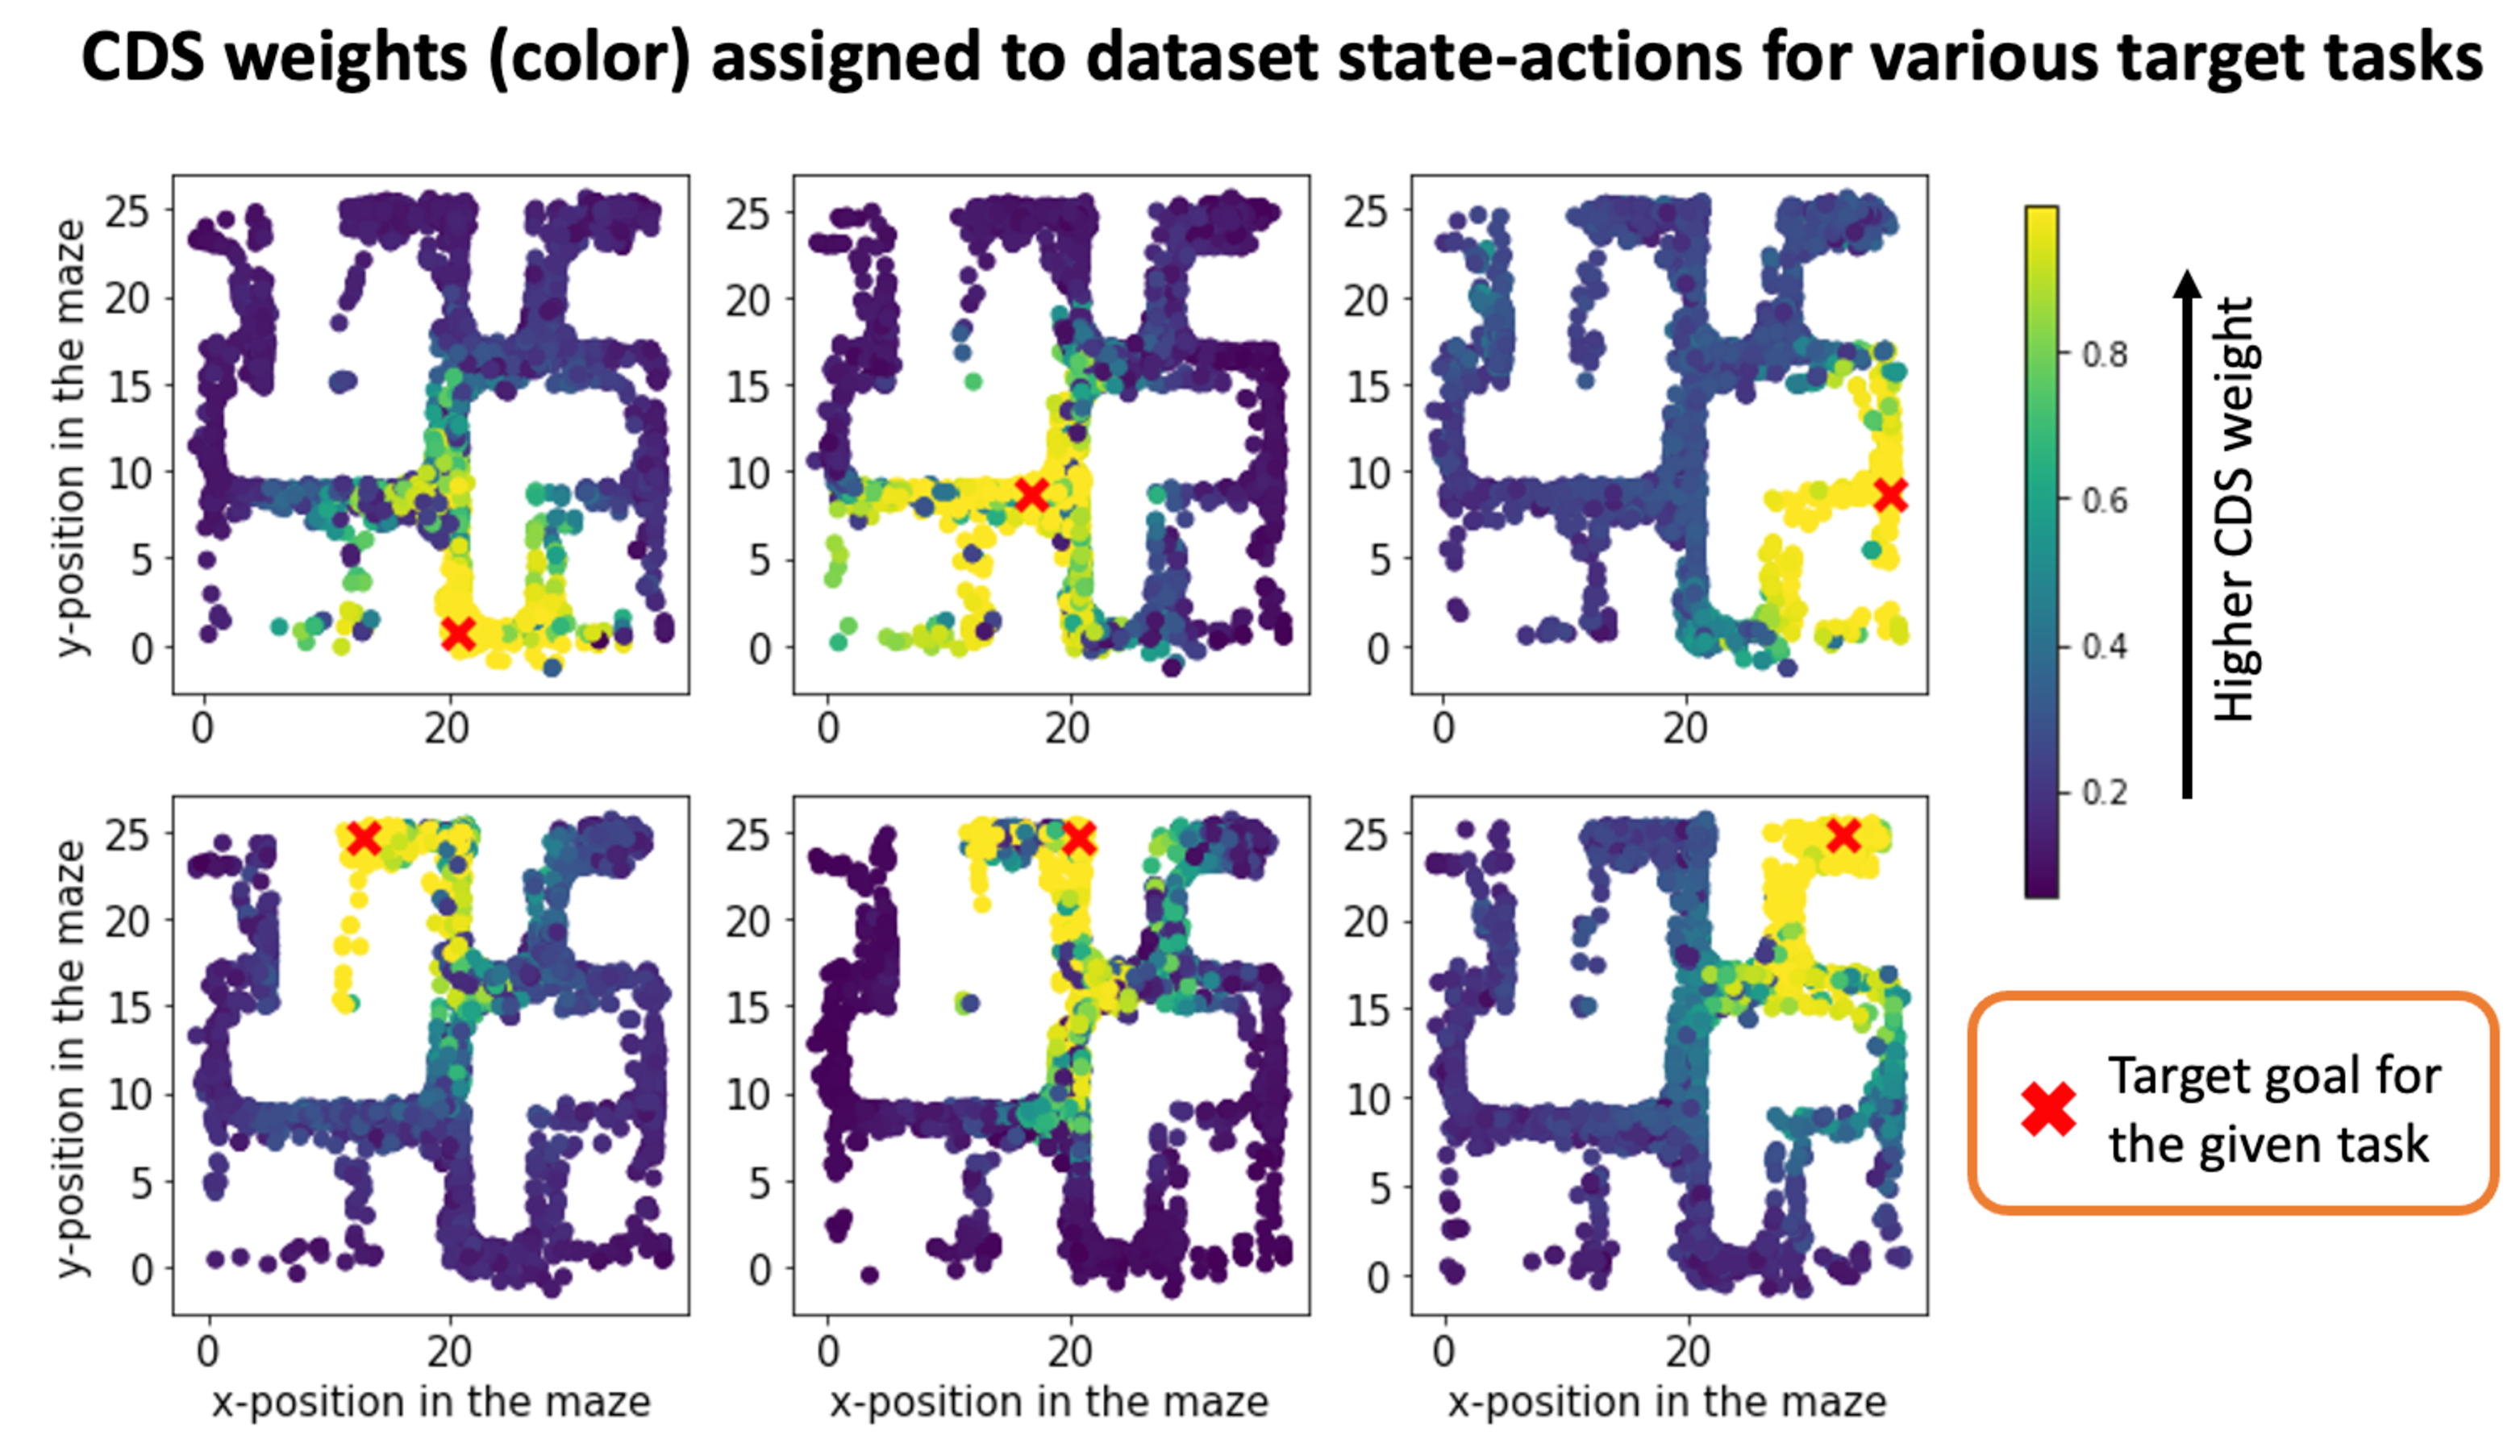
\includegraphics[width=0.75\textwidth]{antmaze_visualization_cds.pdf}
    \vspace{-0.2cm}
    \caption{\footnotesize A visualization of the weights assigned by \methodname\ to various transitions in the antmaze dataset for six target goals (indicated by \textcolor{red}{$\times$} clustered by their spatial location. Note that CDS up-weights transitions spatially close to the target goal (indicated in the brighter yellow color), matching our expectation.}
    \label{fig:antmaze_vis}
    \vspace{-0.4cm}
\end{figure}

Finally, we aim to empirically verify how other alternatives to data sharing perform on multi-task offline RL problems. One simple approach to utilize data from other tasks is to use this data to learn low-dimensional representations that capture meaningful information about the environment initially in a pre-training phase and then utilize these representations for improved multi-task RL without any specialized data sharing schemes. To assess the efficacy of this alternate approach of using multi-task offline data, in Table~\ref{tbl:pretrain_comparison}, we performed an experiment on the Meta-World domain that first utilizes the data from all the tasks to learn a shared representation using the best method, ACL~\citep{yang2021representation} and then runs standard offline multi-task RL on top of this representation. We denote the method as \textbf{Offline Pretraining}. We include the average task success rates of all tasks in the table below. While the representation learning approach improves over standard multi-task RL without representation learning (\textbf{No Sharing}) consistent with the findings in \citep{yang2021representation}, we still find that CDS with no representation learning outperforms this representation learning approach by a large margin on multi-task performance, which suggests that conservative data sharing is more important than pure pretrained representation from multi-task datasets in the offline multi-task setting. We finally remark that in principle, we could also utilize representation learning approaches in conjunction with data sharing strategies and systematically characterizing this class of hybrid approaches is a topic of future work.}

\begin{table*}[t!]
\centering
\vspace*{0.1cm}
\scriptsize
\resizebox{\textwidth}{!}{\begin{tabular}{l|l|r|r|r}
\toprule
\textbf{Environment} & \textbf{Tasks / Dataset type} & \textbf{\methodname\ (ours)} & \textbf{No Sharing} & \textbf{Offline Petraining~\citep{yang2021representation}}\\ \midrule
& door open / expert & \textbf{58.4\%}$\pm$9.3\% & 14.5\%$\pm$12.7\% & 48.0\%$\pm$40.0\%\\
& door close / medium-replay & \textbf{65.3\%}$\pm$27.7\% & 4.0\%$\pm$6.1\% & 9.5\%$\pm$8.4\% \\
Meta-World~\citep{yu2020metaworld}& drawer open / medium-replay & \textbf{57.9\%}$\pm$16.2\% & 16.0\%$\pm$17.5\% & 1.3\% $\pm$ 1.4\%\\
& drawer close / expert & 98.8\%$\pm$0.7\% & 99.0\%$\pm$0.7\% & 96.0\%$\pm$0.9\%\\
& \CC \textbf{average} & \CC \textbf{70.1\%}$\pm$8.1\% & \CC 33.4\%$\pm$8.3\% & \CC 38.7\%$\pm$11.1\%\\
\bottomrule
\end{tabular}}
\vspace{-0.2cm}
\caption{\footnotesize \arxiv{Comparison between CDS and Offline Pretraining~\citep{yang2021representation} that pretrains the representation from the multi-task offline data and then runs multi-task offline RL on top of the learned representation on the Meta-World domain. Numbers are averaged across 6 seeds, $\pm$ the 95$\%$-confidence interval. \methodname\ significantly outperforms Offline Pretraining.}
}
\label{tbl:pretrain_comparison}
\normalsize
\vspace{-0.3cm}
\end{table*}

% \begin{table*}[t!]
% \centering
% \vspace*{0.1cm}
% \scriptsize
% \resizebox{\textwidth}{!}{\begin{tabular}{l|l|r|r|r|r|r|r}
% \toprule
% \textbf{Environment} & \textbf{Tasks / Dataset type} & \textbf{\methodname\ (ours)} & \textbf{\methodname\ (basic)} & \textbf{HIPI}~\cite{eysenbach2020rewriting}& \textbf{Sharing All} & \textbf{No Sharing} & \textbf{Offline Petraining~\citep{yang2021representation}}\\ \midrule
% & door open / medium-replay & \textbf{58.4\%}$\pm$9.3\% & 30.1\%$\pm$16.6\% & 26.5\%$\pm$20.5\% & 34.3\%$\pm$17.9\% & 14.5\%$\pm$12.7 & 7.7\%$\pm$9.3\%\\
% & door close / expert & \textbf{65.3\%}$\pm$27.7\% & 41.5\%$\pm$28.2\% & 1.3\%$\pm$5.3\% & 48.3\%$\pm$27.3\% & 4.0\%$\pm$6.1\% & 48.0\%$\pm$40.0\%\\
% Meta-World~\citep{yu2020metaworld}& drawer open / expert & \textbf{57.9\%}$\pm$16.2\% & 39.4\%$\pm$16.9\% & 41.2\%$\pm$24.9\% & 55.1\%$\pm$9.4\% & 16.0\%$\pm$17.5\% & 1.3\% $\pm$ 1.4\%\\
% & drawer close / medium-replay & 98.8\%$\pm$0.7\% & 86.3\%$\pm$0.9\% & 62.2\%$\pm$33.4\% & \textbf{100.0\%}$\pm$0\% & 99.0\%$\pm$0.7\% & 96.0\%$\pm$0.9\%\\
% & \CC \textbf{average} & \CC \textbf{70.1\%}$\pm$8.1\% & \CC 49.3\%$\pm$16.0\% & \CC 32.8\%$\pm$18.7\% & \CC 59.4\%$\pm$5.7\% & \CC 33.4\%$\pm$8.3\% & \CC 38.7\%$\pm$11.1\%\\
% \bottomrule
% \end{tabular}}
% \vspace{-0.2cm}
% \caption{\footnotesize \arxiv{Comparison between CDS and Offline Pretraining~\citep{yang2021representation} that pretrains the representation from the multi-task offline data and then runs multi-task offline RL on top of the learned representation on the Meta-World domain. Numbers are averaged across 6 seeds, $\pm$ the 95$\%$-confidence interval. \methodname\ significantly outperforms Offline Pretraining.}
% }
% \label{tbl:pretrain_comparison}
% \normalsize
% \vspace{-0.3cm}
% \end{table*}

% \begin{table*}[t!]
% \centering
% \vspace*{0.1cm}
% \scriptsize
% \begin{tabular}{l|l|r|r|r|r}
% \toprule
% \textbf{Environment} & \textbf{Tasks / Dataset type} & \textbf{\methodname\ (ours)}& \textbf{HIPI}~\cite{eysenbach2020rewriting}& \textbf{Sharing All} & \textbf{No Sharing}\\ \midrule
% & run forward / medium-replay & 2587.7$\pm$3.4  & \textbf{2626.1}$\pm$4.2 & 2605.0$\pm$1.2 & \textbf{2632.5}$\pm$1.2\\
% halfcheetah & run backward / medium & 2519.5$\pm$32.0  & \textbf{2634.4}$\pm$1.2 & \textbf{2636.7}$\pm$1.2 & \textbf{2630.7}$\pm$35.6\\
% & jump / expert & \textbf{4298.2}$\pm$66.6 & 4113.4$\pm$78.1 & 712.3$\pm$1874.6 & -1978.3$\pm$3573.9\\
% & \CC \textbf{average} & \CC \textbf{3135.1}$\pm$14.2 & \CC \textbf{3124.7}$\pm$27.0 & \CC 1984.7$\pm$616.6 & \CC 1095.0$\pm$1191.6\\
% \midrule
% & run forward / medium-replay & \textbf{1100.7}$\pm$473.3 & 692.2$\pm$73.3 & 701.4$\pm$63.2 & 590.1$\pm$30.5\\
% walker2d & run backward / medium & 638.4$\pm$82.6 & 664.9$\pm$24.3& \textbf{756.7}$\pm$15.6& 614.7$\pm$34.7\\
% & jump / expert & 1538.4$\pm$290.7  & \textbf{1604.4}$\pm$85.5 & 885.1$\pm$116.0 & 1575.2$\pm$113.0\\
% & \CC \textbf{average} & \CC \textbf{1092.5}$\pm$148.2 & \CC 987.2$\pm$37.1 & \CC 781$\pm$57.2 & \CC 926.6$\pm$46.4\\\midrule
% & run forward / medium-replay & 2350.1$\pm$91.9 & \textbf{2658.9}$\pm$63.4 & 1175.0$\pm$184.5 & 2126.7$\pm$160.3\\
% ant & run backward / medium & 1435.7$\pm$70.7 & 1208.2$\pm$64.7 & 1488.7$\pm$142.4 & \textbf{2021.7}$\pm$14.1\\
% & jump / expert & \textbf{2781.3}$\pm$392.6 & 2670.4$\pm$61.0 & 133.8$\pm$678.2 & 495.8$\pm$134.9\\
% & \CC \textbf{average} & \CC \textbf{2189.0}$\pm$107.9 & \CC \textbf{2179.2}$\pm$9.7 & \CC 932.5$\pm$179.7 & \CC 1548.1$\pm$84.1\\
% \midrule
% & door open / medium-replay & \textbf{57.3\%}$\pm$17.2\% & 30.7\%$\pm$43.4\% & 19.1\%$\pm$25.2\% & 0\%$\pm$0\%\\
% & door close / expert & \textbf{33.3\%}$\pm$18.0\% & 0\%$\pm$0\% & 21\%$\pm$25.9\% & 2\%$\pm$2.8\% \\
% Meta-World~\citep{yu2020metaworld}& drawer open / expert & 76\%$\pm$9.3\%  & 45.3\%$\pm$32.2\% & \textbf{85.5\%}$\pm$7.3\% & 0\%$\pm$0\%\\
% & drawer close / medium-replay & 99.7\%$\pm$0.5\% & 66.7\%$\pm$47.1\% & \textbf{100\%}$\pm$0\% & 5.7\%$\pm$4.9\%\\
% & \CC \textbf{average} & \CC \textbf{66.6\%}$\pm$9.1\% & \CC 35.7\%$\pm$26.6\% & \CC 56.4\%$\pm$7.5\% & \CC 1.9\%$\pm$0.8\%\\
% \midrule
% & large maze (7 tasks) / undirected & \textbf{0.23} $\pm$ 0.17 & 0.01 $\pm$ 0.00 & 0.17 $\pm$ 0.12 & 0.13 $\pm$ 0.09 \\
% AntMaze~\citep{fu2020d4rl}  & large maze (7 tasks) / directed & \textbf{0.24} $\pm$ 0.05 & 0.12 $\pm 0.07$ & \textbf{0.21} $\pm$ 0.08 & \textbf{0.23} $\pm$ 0.20 \\
% & medium maze (3 tasks) / undirected & \textbf{0.37} $\pm$ 0.11 & 0.07 $\pm$ 0.00 & 0.23 $\pm$ 0.15 & 0.22 $\pm$ 0.12\\
% & medium maze (3 tasks) / directed & \textbf{0.19} $\pm$ 0.08 & 0.08 $\pm$ 0.00 & 0.12 $\pm$ 0.10 & \textbf{0.17} $\pm$ 0.20 \\
% \bottomrule
% \end{tabular}
% %%CF.6.3: Are you going to provide error bars for ant maze? if not, I would just omit it from this table.
% \vspace{-0.2cm}
% \caption{\footnotesize Results for multi-task locomotion, robotic manipulation and navigation environments with low-dimensional state inputs. On locomotion environments (halfcheetah, walker2d and ant), we include three tasks, run forward, run backward and jump, are provided in each environment. We use medium-replay datasets for task run forward, medium datasets for task run backward, and expert datasets with limited data for task jump. On the multi-task robotic manipulation domain, we consider four tasks from Meta-World~\citep{yu2020metaworld}, door open, door close, drawer open and drawer close with medium-replay, expert, medium-replay and expert datasets respectively. Similar to locomotion tasks, we also used limited amount of expert trajectories for the expert dataset. On the antmaze navigation task, we consider two maze layouts (medium/large) from D4RL~\citep{fu2020d4rl}, and distribute existing D4RL data either randomly across tasks (undirected) or based on relevance of the trajectory in the dataset to the task of interest (directed). Reported is the average return for locomotion tasks, normalized score as proposed in \citep{fu2020d4rl} for AntMaze or success rate for Meta-World environments, averaged over 3 random seeds, $\pm$ 1 standard deviation. We include both per-task performance and the overall performance averaged across tasks (highlighted in gray). We bold the highest score across all methods as well as methods with scores within 1\% range of the mean of the highest score except that in the directed setting on AntMaze, we bold  \methodname\ , \textbf{No Sharing} and/or \textbf{Sharing All} due to the similar mean score and large standard deviation. \methodname\ performs achieves the best or comparable performance on all of these multi-task environments.
% }
% \label{tbl:low_dim_full}
% \normalsize
% \vspace{-0.2cm}
% \end{table*}

% Additionally, we also provide the full table of the empirical analysis as discussed in Section~\ref{sec:analysis}. In Table~\ref{tab:analysis_full}, we provide 

% \begin{table*}[t]
%   \centering
%   \scriptsize
%   \def\arraystretch{0.9}
%   \setlength{\tabcolsep}{0.42em}
% \begin{tabularx}{0.9\linewidth}{cc*{6}{c}}
%   \toprule
%  \multicolumn{1}{c}{\multirow{1.5}[2]{*}{Dataset types}} & \multicolumn{1}{c}{\multirow{1.5}[2]{*}{Tasks}} &
%  \multicolumn{2}{c}{No Sharing} & \multicolumn{2}{c}{Sharing All}  & \multicolumn{2}{c}{CDS (ours)}\\
% & \multicolumn{1}{c}{} & \multicolumn{1}{c}{Avg Return}  & \multicolumn{1}{c}{$D_\text{KL}(\pi, \pi_\beta)$}  & \multicolumn{1}{c}{Avg Return}  & \multicolumn{1}{c}{$D_\text{KL}(\pi, \pi_\beta)$} & \multicolumn{1}{c}{Avg Return}  & \multicolumn{1}{c}{$D_\text{KL}(\pi, \pi_\beta)$} \\
% \midrule
%   medium-replay & run forward & 998.9 & \textbf{3.70} & 966.2 & 10.39 & \textbf{1136.5} & 11.27\\
%   medium-replay & run backward & 1298.6 & \textbf{4.55} & 1147.5 & 12.70 & \textbf{1649.4} & 8.68\\
%   medium-replay & jump & \textbf{1603.1} & \textbf{3.57} & 1224.7 & 15.89 & 1320.0 & 9.32\\
%   & average task results & 1300.2 &  & 1112.8 &  & \textbf{1368.6} &\\
%   \midrule
%   medium & run forward & 297.4 & \textbf{6.53} & 848.7 & 11.78 & \textbf{933.2} & 6.91\\
%   medium & run backward & 207.5 & \textbf{4.44} & 600.4 & 10.13 & \textbf{877.4} & 6.38\\
%   medium & jump & 351.1 & 5.57 & 776.1 & 21.27 & \textbf{1334.5} & \textbf{5.56}\\
% %   \hline
%   & average task results & 285.3 &  & 747.7 & & \textbf{933.2} &\\
%   \midrule
%   medium-replay & run forward & 590.1 & \textbf{1.49} & 701.4 & 7.76 & \textbf{1100.7} & \textbf{1.49}\\
%   medium & run backward & 614.7 & \textbf{1.91} & \textbf{756.7} & 12.2 & 638.4 & 6.09\\
%   \rowcolor{Gray}
%   expert & jump & \textbf{1575.2} & 3.12 & 885.1 & 27.5 & 1538.4 & \textbf{2.91}\\
% %   \hline
%   & average task results & 926.6 &  & 781 &  & \textbf{1092.5} & \\
%   %%CF.5.22: is this the average for all tasks or just the last three?
%     \bottomrule
%     \end{tabularx}
%     \vspace{-0.2cm}
%          \caption{\footnotesize Empirical analysis
%          %%CF.5.22: need more detail.
%          %%CF.5.22: definitely need to describe what the KL column corresponds to.
%      \label{tab:analysis_full}
%      }
% \end{table*}